\documentclass[12pt]{article}
\usepackage[utf8]{inputenc}

\usepackage{enumerate}
\usepackage{listings}
\usepackage{pgfplots}
\usepackage{tikz}
\usepackage{svg}
\usepackage{graphicx}
\usepackage{setspace}
\usepackage{makecell}
\usepackage{caption}
\usepackage{subcaption}
\usepackage{pgf-umlsd}
\usepackage{epstopdf}
\usepackage{bytefield}
\usepackage{amsmath}
\usepackage{csquotes}
\usepackage[nottoc,numbib]{tocbibind}
\usepackage[section]{placeins}
\usepackage{tgtermes}
\usepackage{color}
\usepackage{hyperref}

\usetikzlibrary{shapes.geometric}
\usetikzlibrary{decorations.text}
\usetikzlibrary{positioning}
\usetikzlibrary{fit,shapes}

\hypersetup{
colorlinks,
citecolor=black,
filecolor=black,
linkcolor=black,
urlcolor=black
}

\lstloadlanguages{TeX}

\definecolor{lightred}{rgb}{1,0.7,0.71}

\begin{document}

    \thispagestyle{empty}
{\fontfamily{qtm}\selectfont
\begin{figure}[htbp]
    \centering
    
\includegraphics[scale=1.5]{img/agh-logo.pdf}
\end{figure}

\centerline{\small\textbf{AKADEMIA GÓRNICZO-HUTNICZA IM. STANISŁAWA STASZICA W KRAKOWIE}}
\vspace{1em}
\centerline{\small\textbf{WYDZIAŁ INFORMATYKI, ELEKTRONIKI I TELEKOMUNIKACJI}}
\vspace{1em}
\centerline{\small INSTYTUT Informatyki}
\vspace{2em}
\centerline{\Large Praca dyplomowa}
\vspace{2em}
\centerline{\textit{\large Validation of QUIC protocol usefullness in interactive communication}}
\vspace{1em}
\centerline{\textit{\large Ocena przydatności protokołu QUIC w komunikacji interaktywnej}}
\vspace{3em}

\begin{table}[h]
    \begin{tabular}{l l}
        Autor             & Michał Śledź              \\
        Kierunek studiów: & Informatyka               \\
        Opiekun pracy:    & dr inż.\ Łukasz Czekierda \\
    \end{tabular}
\end{table}

\null
\vfill
\centerline{Kraków, 2021}
}
    \clearpage

    \tableofcontents
    \clearpage

    \section{Introduction}
\label{sec:introduction}

An interactive communication is bidirectional data exchange between people or people and machines.
It consists of two or more participants and has to be responsive meaning the result of performed action is delivered almost immediately.
In many cases interactive communication has to be also secure and reliable.
Examples of interactive communication are controlling remote robot in tele-surgery, doing exercises in tele-rehabilitation and
some types of multimedia sessions e.g.\ video conference, collaborative work or chat.
On the other hand to interactive communication does not belong exchanging emails (time between subsequent messages is too big) or
video on demand and streaming (they are not bidirectional).

Years of researches, protocol improvements and network devices optimizations have made interactive communication really fast.
We can talk with another person almost in the real time with a delay of several milliseconds.
Having said that it is perfectly correct to ask a question whether communication can be even faster, more effective and reliable and whether it is still worth to make improvements while we already have well prospering ecosystem.
In 2006 Prof.\ Edward Delp said:
\begin{displayquote}
    Is video coding dead?
    Some feel that, with the higher coding efficiency of the H.264/MPEG-4 Advanced Video Coding (AVC) standard (2x as compared to MPEG-2), perhaps there is not much more to do.
    I must admit that I have heard this \textquote{compression is dead} argument at least four times since I started working in image and video coding in 1976.\cite{4015574}
\end{displayquote}
Despite the fact that we are able to achieve very good performance in video conferencing systems there is still much to do.
Serious gaming, tele-surgery and tele-rehabilitation are all subject to tactile internet in which reliability, security and low latency are fundamental.
In such cases delay of 1 ms is desirable~\cite{the-tactile-internet}.

On the other hand, complexity of current standards makes them hard to implement, monitor and maintain.
One of them is WebRTC which uses over 10 different protocols and leaves implementation of signalling plane to the user.

QUIC is a new transport protocol standardized in RFC 9000 on May in 2021 and provides interesting and promising set of features.
%Its integration with TLS 1.3 significantly reduces connection establishment time while stream multiplexing in a single connection resolves head of line blocking problem of HTTP/2.
%QUIC introduces also special connection identifiers that prevents from additional handshakes in case of network switching and defines own flow control and congestion control mechanisms that are based on TCP ones.
%QUIC packets are encapsulated in UDP datagrams which makes QUIC user level protocol i.e.\ there is no need to modify kernel implementation to provide operating system with support for QUIC\@.
%
QUIC is mostly deployed in conjunction with a new version of HTTP called HTTP/3 and is intended to replace TCP and HTTP/2.
Therefore most publications are focused on web domain comparing QUIC and HTTP/3 with TCP/TLS and HTTP/2.

However, it turns out that a lot of QUIC features mainly stream multiplexing, pluggable congestion control, integration with TLS 1.3
or enhanced connection establishment mechanism can be useful in other domains.
As a result a number of IETF drafts emerged to expand QUIC to new areas.
The most important one is \textit{An Unreliable Datagram Extension to QUIC}.
It allows for combining reliable and unreliable data exchange in the same QUIC connection.

This document tries to answer a question whether QUIC can introduce significant improvement in terms of interactive communication.
To this end, analysis of QUIC encryption, loss detection and flow control mechanisms as well as number of tests and experiments have been performed.

The structure of this document is as follows.
Section~\ref{sec:state-of-the-art} presents state of the art and defines problems that will be addressed in this document.
Section~\ref{sec:quic-overview} introduces basic concepts of QUIC and compares QUIC to other transport protocols.
Section~\ref{sec:quic-in-webrtc} presents how QUIC can simplify WebRTC protocol stack.
It also describes packet encryption process in QUIC, answers the question if header encryption introduces significant overhead to the whole packet encryption and compares QUIC encryption process with RTP one.
Section~\ref{sec:datagrams} is dedicated to DATAGRAM frames in QUIC -- how they work and behave in different scenarios.
Section~\ref{sec:conclusions} concludes this document.

    \clearpage
    %! suppress = EscapeAmpersand


\section{QUIC overview}
\label{sec:quic-overview}
QUIC is a connection-based, multistream protocol that uses UDP under the hood.
It is integrated with TLS and provides own congestion control and flow control mechanisms.
Data sent over QUIC is delivered in a reliable, ordered way.
Together with QUIC there comes a new version of HTTP called HTTP/3.

This section outlines main features of QUIC and compares QUIC to the other transport protocols.

\subsection{Packet types in QUIC}
\label{subsec:quic-packet-types}
The most outer entity in QUIC is a packet.
Each QUIC packet consists of a header that can take long or short form and one or more QUIC frames.
QUIC packets are directly encapsulated into UDP datagrams.
This is illustrated in figure~\ref{fig:quic-packet-format}.
A single UDP datagram can also coalesce many QUIC packets, however, this feature is not important in terms of regular data exchange.

\begin{figure}
    \centering
    \begin{bytefield}{32}
        \begin{leftwordgroup}{\tiny UDP header}
            \bitbox{16}{\tiny source port} & \bitbox{16}{\tiny destination port} \\
            \bitbox{16}{\tiny length} & \bitbox{16}{\tiny checksum}
        \end{leftwordgroup} \\
        \begin{leftwordgroup}{\tiny UDP data}
            \begin{rightwordgroup}{\tiny QUIC packet}
                \wordbox{1}{\tiny quic header} \\
                \wordbox[tlr]{1}{\tiny  quic frames} \\
                \wordbox[blr]{1}{\tiny $\cdots$}
            \end{rightwordgroup}
        \end{leftwordgroup}
    \end{bytefield}
    \caption{QUIC packet format}
    \label{fig:quic-packet-format}
\end{figure}

QUIC defines two types of header: short and long.
Figure~\ref{fig:short-header-format} illustrates Short Header format.
The first byte encodes miscellaneous flags.
Next, there is a destination connection ID that takes at most 20 bytes and a packet number that takes from 1 to 4 bytes.
Total size of Short Header is from 2 to 25 bytes.
Fields marked with red color are subject to an encryption process.
On the other hand Long Header additionally includes version, destination connection ID length, source connection ID length and source connection ID\@.
Flags differ a little comparing to the Short Header but together with a packet number length they also take 1 byte.

\begin{figure}
    \centering
    \begin{bytefield}[bitwidth=4em]{8}
        \bitheader{0-7} \\
        \bitbox{1}{\tiny header form} & \bitbox{1}{\tiny fixed bit} & \bitbox{1}{\tiny spin bit} & \bitbox{2}[bgcolor=lightred]{\tiny reserved bits} & \bitbox{1}[bgcolor=lightred]{\tiny key phase} & \bitbox{2}[bgcolor=lightred]{\tiny packet number length} \\
        \wordbox{1}{\tiny destination connection ID (0 - 160)} \\
        \wordbox{1}[bgcolor=lightred]{\tiny packet number (8 - 32)}
    \end{bytefield}
    \caption{QUIC Short Header format}
    \label{fig:short-header-format}
\end{figure}

QUIC introduces also different types of packets and frames.
Depending on specific packet type, it can contain different frame types.
For example \textit{Handshake} packet can contain \textit{CRYPTO}, \textit{PING}, \textit{PADDING}, \textit{ACK} or \textit{CONNECTION\_CLOSE} frames.
We can divide packet types basing on header form they use.
Following packet types use Long Header: \textit{Version Negotiation}, \textit{Initial}, \textit{0-RTT}, \textit{Handshake}, \textit{Retry}.
They are sent at the beginning of communication and therefore they are not covered more here.

Packet that uses Short Header is called \textit{1-RTT}.
1-RTT packets are sent after version and 1-RTT keys negotiation.
In an interactive communication they are main packets and they will, for example, convey media data.
1-RTT packet format is illustrated in figure~\ref{fig:1rtt-packet-format}.

\begin{figure}
    \centering
    \begin{bytefield}[bitwidth=3.5em]{8}
        \bitheader{0-7} \\
        \begin{leftwordgroup}{\tiny short \\ \tiny header}
            \bitbox{1}{\tiny header form} & \bitbox{1}{\tiny fixed bit} & \bitbox{1}{\tiny spin bit} & \bitbox{2}[bgcolor=lightred]{\tiny reserved bits} & \bitbox{1}[bgcolor=lightred]{\tiny key phase} & \bitbox{2}[bgcolor=lightred]{\tiny packet number length} \\
            \wordbox{1}{\tiny destination connection ID (0 - 160)} \\
            \wordbox{1}[bgcolor=lightred]{\tiny packet number (8 - 32)}
        \end{leftwordgroup} \\
        \wordbox[tlr]{1}[bgcolor=lightred]{\tiny payload} \\
        \wordbox[blr]{1}[bgcolor=lightred]{\tiny $\cdots$}
    \end{bytefield}
    \caption{QUIC 1-RTT packet format}
    \label{fig:1rtt-packet-format}
\end{figure}

\subsection{Security and low-latency connection establishment}
\label{subsec:security-and-low-latency-connection-establishment}
QUIC is integrated with TLS 1.3 providing confidentiality, integrity and authenticity of its packets.
Integration with TLS 1.3 is described in details in RFC 9001~\cite{rfc9001}.
It is based on negotiating both transport and cryptographic parameters in a single connection handshake which results in a low-latency connection establishment.
Figure~\ref{fig:low-latency-conn-est} compares time needed for sending HTTP request using TCP/TLS and QUIC\@.

\begin{figure}
    \centering
    \begin{subfigure}{.5\textwidth}
        \begin{sequencediagram}
            \newinst{client}{Client}
            \newinst[3]{server}{Server}
            \mess{client}{TCP SYN}{server}
            \mess{server}{TCP SYN + ACK}{client}
            \mess{client}{TCP ACK}{server}
            \postlevel
            \mess{client}{TLS ClientHello}{server}
            \mess{server}{TLS ServerHello}{client}
            \mess{client}{TLS Finished}{server}
            \postlevel
            \mess{client}{HTTP REQ}{server}
            \mess{server}{HTTP RES}{client}
        \end{sequencediagram}
        \caption{HTTP request in TCP}
        \label{subfig:http-req-tcp}
    \end{subfigure}%
    \begin{subfigure}{.5\textwidth}
        \begin{sequencediagram}
            \newinst{client}{Client}
            \newinst[3]{server}{Server}
            \mess{client}{QUIC}{server}
            \mess{server}{QUIC}{client}
            \mess{client}{QUIC}{server}
            \postlevel
            \mess{client}{HTTP REQ}{server}
            \mess{server}{HTTP RES}{client}
        \end{sequencediagram}
        \caption{HTTP request in QUIC}
        \label{subfig:http-req-quic}
    \end{subfigure}
    \caption{HTTP request comparison between TCP/TLS and QUIC}
    \label{fig:low-latency-conn-est}
\end{figure}

Round Trip Time (RTT) is a time needed for transporting a message from one side to the other and back again.
Standard HTTP request using TCP/TLS stack requires 3-RTT -- one for TCP handshake, one for TLS handshake and one for HTTP request.
Even though TCP handshake sends 3 messages it is still counted as 1-RTT because we do not have to wait for a response to the last message but we can immediately send next data, which in this case is data for TLS handshake.

QUIC takes another approach.
It combines transport and cryptographic handshakes reducing time needed for establishing a connection.
In such a case sending an HTTP request occurs after 1-RTT\@.
The whole communication lasts 2-RTT\@.

However, QUIC can reduce time needed for sending an HTTP request and receiving a response even more.
In case when there was communication with the server previously and client cached information from it, it is possible to send 0-RTT HTTP request.
This scenario is presented in figure~\ref{fig:http-req-quic-0rtt}
\begin{figure}
    \centering
    \begin{sequencediagram}
        \newinst{client}{Client}
        \newinst[3]{server}{Server}
        \mess{client}{QUIC}{server}
        \mess{client}{HTTP REQ}{server}
        \postlevel
        \mess{server}{QUIC}{client}
        \mess{server}{HTTP RES}{client}
        \postlevel
        \mess{client}{QUIC}{server}
    \end{sequencediagram}
    \caption{HTTP request in QUIC with 0-RTT packets}
    \label{fig:http-req-quic-0rtt}
\end{figure}

The only limitation of integrating TLS with QUIC is that there is no possibility to send unencrypted data.

\FloatBarrier

\subsection{Stream multiplexing}
\label{subsec:stream-multiplexing}
QUIC is a multiplexed protocol which means we can open many streams in one QUIC connection.
Stream is an ordered sequence of bytes.
Each stream can be unidirectional or bidirectional and can be opened by a client or by a server.
Different types of streams can have different flow control limits (see section~\ref{subsec:flow-control-and-congestion-control}).
Data in specific streams is carried independently which means that losing packet in one stream does not affect flow in other streams.
Figure~\ref{fig:stream-multiplexing} shows this scenario.
One of the packets in stream 1 (marked as gray) was lost and needs to be retransmitted blocking subsequent packets (marked as black) on the receiver side.
They cannot be conveyed to the application layer until retransmission and reordering of the lost packet.
This is the source of so called head of line blocking problem which appears when we are trying to multiplex many HTTP requests in a single TCP connection.
Losing one packet stops the entire flow.
However, thanks to the stream multiplexing QUIC resolves this problem and streams 2 and 3 are not affected by the packet loss in stream 1.

\begin{figure}
    \centering
    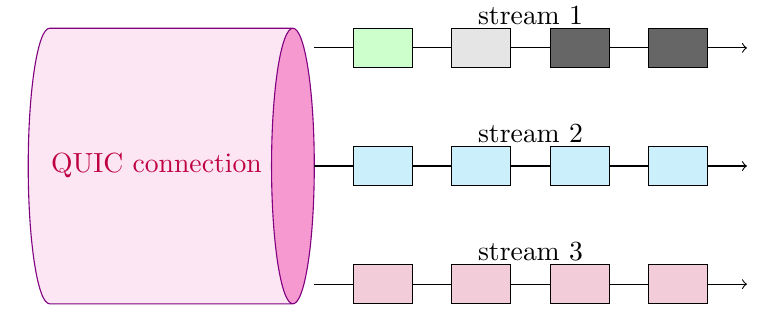
\begin{tikzpicture}

        \node[cylinder,
        draw = violet,
        text = purple,
        style={transform shape},
        cylinder uses custom fill,
        cylinder body fill = magenta!10,
        cylinder end fill = magenta!40,
        minimum size = 3.5cm] (c) at (0,0) {QUIC connection};

        \draw [->, postaction={decorate,decoration={raise=2ex, text along path,text align=center,text={stream 1}}}] (2, 1.5) -- (7.5, 1.5);
        \filldraw [fill=green!20, draw=black] (2.5, 1.25) rectangle (3.25, 1.75);
        \filldraw [fill=gray!20, draw=black] (3.75, 1.25) rectangle (4.5, 1.75);
        \filldraw [fill=black!60, draw=black] (5, 1.25) rectangle (5.75, 1.75);
        \filldraw [fill=black!60, draw=black] (6.25, 1.25) rectangle (7, 1.75);

        \draw [->, postaction={decorate,decoration={raise=2ex, text along path,text align=center,text={stream 2}}}] (2, 0) -- (7.5, 0);
        \filldraw [fill=cyan!20, draw=black] (2.5, -0.25) rectangle (3.25, 0.25);
        \filldraw [fill=cyan!20, draw=black] (3.75, -0.25) rectangle (4.5, 0.25);
        \filldraw [fill=cyan!20, draw=black] (5, -0.25) rectangle (5.75, 0.25);
        \filldraw [fill=cyan!20, draw=black] (6.25, -0.25) rectangle (7, 0.25);

        \draw [->, postaction={decorate,decoration={raise=2ex, text along path,text align=center,text={stream 3}}}] (2, -1.5) -- (7.5, -1.5);
        \filldraw [fill=purple!20, draw=black] (2.5, -1.75) rectangle (3.25, -1.25);
        \filldraw [fill=purple!20, draw=black] (3.75, -1.75) rectangle (4.5, -1.25);
        \filldraw [fill=purple!20, draw=black] (5, -1.75) rectangle (5.75, -1.25);
        \filldraw [fill=purple!20, draw=black] (6.25, -1.75) rectangle (7, -1.25);


    \end{tikzpicture}
    \caption{Stream multiplexing in a single QUIC connection}
    \label{fig:stream-multiplexing}
\end{figure}

\subsection{Connection migration}
\label{subsec:connection-migration}
Each QUIC connection has a set of connection identifiers each of which can identify the connection.
Connection IDs can be variable length.
QUIC uses connection IDs to route packets to proper endpoint.
This way, as long as there is an alternative network path, QUIC is resilient to network changes avoiding restarting the connection when an endpoint changes its transport address (IP or port).

\subsection{Flow control and congestion control mechanisms}
\label{subsec:flow-control-and-congestion-control}
Flow control limits amount of data that can be sent to the receiver.
Receiver can announce how much data it is able to process/buffer and sender must not exceed this limit until it is updated.
In QUIC, flow control limits can be set on two levels.
The first one is stream level.
This limit is set per stream type e.g.\ for all unidirectional streams opened by the peer or for all bidirectional streams opened locally.
There is no possibility to set flow control limit for a stream with a particular id.
The second one is connection level and it limits overall data amount that can be sent within the whole connection across all streams.
QUIC allows also for limiting number of streams that can be opened by the peer.
These limits are also set per stream type -- unidirectional or bidirectional and initiated by a peer or locally.

On the other hand congestion control limits amount of data that can be sent through the network.
Whenever there is a danger that some middle-boxes like routers can be overwhelmed by the amount of data they have to process, they require sender to slow down its transmission rate.
This is often done using ECN (Explicit Congestion Notification) flag in an IP packet.
RFC 9001~\cite{rfc9001} defines congestion controller similar to TCP NewReno.
However, any other congestion controller that meets requirements defined in section 3.1 of RFC 8085~\cite{rfc8085} can be used.
This makes QUIC congestion control mechanism pluggable.

\subsection{Reliability}
\label{subsec:reliability}
QUIC is a reliable protocol which means it guarantees delivery of each packet sent by the endpoint.
Packets are delivered to the receiver side in the order they were sent.
However, there are different IETF drafts that expand QUIC with new features.
One of them called \textit{An Unreliable Datagram Extension to QUIC}\cite{bider-ssh-quic-09} allows for sending unreliable messages over QUIC\@.
This can take place in simultaneously to the reliable communication.
Unreliable messages are not subject to flow control mechanisms however, they are congestion controlled.
Each unreliable message is also acknowledged so that application layer can be provided with the packet loss information.
Section~\ref{sec:datagrams} describes Datagram extension in details.

\subsection{QUIC against other transport protocols}
\label{subsec:quic_against_other_transport_protocols}
This section compares QUIC with three main transport protocols -- TCP, UDP and SCTP\@.

\subsubsection{TCP}
Transmission Control Protocol -- connection based, stream oriented and reliable transport protocol.
It guarantees the order of messages and provides flow control and congestion control mechanisms.
TCP is not a multiplexed protocol.
In one TCP connection we have one logical communication channel.
This is the reason of head of line blocking problem that appears when many HTTP/2 requests are multiplexed in one TCP connection.
Because of its reliability, TCP is not a good choice for many types of interactive communication.

\subsubsection{UDP}
User Datagram Protocol -- connection less, unreliable transport protocol.
It does not preserve the order of messages.
Datagrams, in this protocol, are not acknowledged nor congestion controlled.
It does not also introduce any flow control mechanisms.
Thanks to its simplicity and low bandwidth affection it is the base for RTP protocol which is widely used for transmitting multimedia.
Unlike TCP, UDP also allows for multicast transmission.
However, multicast is rarely used, mostly in local networks.

\subsubsection{SCTP}
Stream Control Transmission Protocol -- reliable, based on UDP, message oriented transport protocol.
Unlike TCP, SCTP is multistream protocol.
SCTP is partially ordered but it also allows for sending unordered messages.
Another feature of SCTP is multi-homing in which an endpoint uses two different addresses.
This introduces some kind of fault tolerance -- one address is designated as a primary and the other one can be used in case of failure of the first one.
Unfortunately SCTP is not widely used.
Its main domain is telecommunication as a lot of home routers does not handle it properly.

\subsubsection{Summary}
Table~\ref{tab:protocols_comparision} presents a short summary of transport protocols comparison.
\begin{table}[h]
    \centering
    \resizebox{\columnwidth}{!}{%
    \begin{tabular}{|c | c | c | c | c |}
        \hline
        & TCP           & UDP              & SCTP              & QUIC          \\
        \hline
        reliability        & reliable      & unreliable       & reliable          & reliable      \\
        \hline
        transmission       & byte oriented & message oriented & message oriented  & byte oriented \\
        \hline
        flow control       & yes           & no               & yes               & yes           \\
        \hline
        congestion control & yes           & no               & yes               & yes           \\
        \hline
        packets order      & ordered       & unordered        & partially ordered & ordered       \\
        \hline
        multistream        & no            & no               & yes               & yes           \\
        \hline
    \end{tabular}%
    }
    \caption{\label{tab:protocols_comparision}Transport protocols comparison.}
\end{table}

    \clearpage
    \section{State of the art}
\label{sec:state-of-the-art}

\textit{The QUIC Fix for Optimal Video Streaming} article~\cite{the-quic-fix-for-optimal-video-streaming} introduces unreliable data transmission over QUIC and presents how combination of reliable and unreliable transmission fares in video streaming and outperforms TCP and reliable mode of QUIC\@.
Authors of this document tag H.264 video frames depending on their importance.
\textit{I-Frames} which are independent frames meaning they can be displayed without any additional frames are marked to be sent reliably.
\textit{P-Frames} which are much smaller in size and code only the difference between \textit{I-Frame} and the next frame are marked to be sent unreliably.
The same approach is applied to \textit{B-Frames} that depends on both \textit{I-Frames} and \textit{P-frames}.
Authors state that the loss of \textit{P-Frames} or \textit{B-Frames} has minimal or no impact on the user's quality of experience (QoE).
They use i.a. \textit{buffering ratio (bufRatio)} and \textit{rate of buffering (rateBuf)} metrics to measure the difference in performance of streaming video over codec-agnostic DASH protocol used with TCP, traditional QUIC and QUIC with addition of unreliable transmission.
\textit{BufRatio} is the amount of time spent on buffering video comparing to the total session time (i.e.\ playing plus buffering time), represented as a percentage.
\textit{RateBuf} is the frequency of the buffering events~\cite{impact-of-video-quality-on-user-engagement}.
As a result, \textit{bufRatio}, with packet loss set to 0.64\%, for TCP is 105\%, for QUIC is 30\% and for QUIC with addition of unreliable data transmission is less than 1\%.
\textit{RateBuf}, with the same packet loss, is equal to 50\% for TCP, 19\% for QUIC and nearly 0\% for QUIC with addition of unreliable data transmission.

\textit{QUIC: Better for what and for whom?} article~\cite{quic-better-for-what-and-for-whom} compares the page load time (PLT) for HTTP/2 requests over QUIC and TCP/TLS in different network conditions and architectures as well as for different website complexities.
Authors prepared both local and remote testbeds.
In the remote one client's machine is connected to the Internet over ADSL (to router over Ethernet or Wi-Fi) or 4G\@.
Different network conditions mean different packet loss rate and delay.
In case of complexity of site there is Youtube service in which different resources might be distributed over many servers and Doctor (website of the ANR project) website where ale files are located on the same server.
Authors concludes that QUIC outperforms HTTP/2 over TCP/TLS in unstable networks but in case of stable and reliable networks the benefits of QUIC are not so obvious.

\textit{Game of protocols: Is QUIC ready for prime time streaming?} article~\cite{game-of-protocols} compares QUIC and TCP in HAS (HTTP adaptive streaming) applications.
To this end, authors performed experiments in four scenarios.
Frame-seek scenario is about seeking to the specified frame in the video.
Connection-switch scenario is about changing the connection from e.g.\ Wi-Fi to 3G\@.
Multiplexing scenario is about comparing different stream multiplexing techniques i.e.\ HTTP/1.1 over varying number of TCP connections, HTTP/2 with parallel requests over a single TCP connection and QUIC over a single UDP connection.
Fairness scenario is about checking fairness of congestion control mechanisms while there are multiple competing clients.
Authors also used three different adaptive algorithms: BASIC, SARA and BBA-2.
In the frame-seek scenario for BASIC algorithm QUIC behaved better by reducing bufRatio (called by authors rebuffer rate) from 3\% for WiFi and LTE to 1\% for WiFi and 2\% for LTE\@.
For 3G networks, QUIC reduced bufRatio from 5\% to 2\%.
For SARA and BBA-2 algorithms the results are also in favor of QUIC\@.
In the WiFi-LTE connection-switch scenario, QUIC reduced numerically bufRatio by 1\%, from 5\% to 4\% for BBA-2, from 4\% to 3\% for SARA and from 3\% to 2\% for BASIC\@.
Average playback bitrates also were a little higher for QUIC\@.
In the WiFi-3G connection-switch scenario, QUIC also behaved better and the reduction of bufRatio was similar except for BASIC algorithm where QUIC reduced bufRatio from 13\% to 6\%.
Evaluation of different multiplexing techniques showed that in the typical network conditions all three methods resulted in the similar average playback bitrate.
In the large delay and typical loss network, QUIC performed best.
For typical delay and large loss as well as for large delay and large loss, HTTP/1.1 with varying number of TCP connections was better than QUIC\@.
HTTP/2 over single TCP connection didn't manage to beat any of the other multiplexing techniques in any of the network conditions.
Fairness examination of congestion control mechanisms in TCP and QUIC showed that for typical packet loss and delay both protocols guarantee fair resource access for competing clients which results in the similar average playback bitrate.
In the large loss scenario single QUIC client was able to achieve higher bitrate (about 37\%) than single TCP client.
For competing clients, QUIC still was able to achieve better bitrate than TCP (about 40\%).
In the large delay scenario, the results were similar to the large loss scenario.
The last one scenario with large loss and large delay showed that TCP client was able to achieve higher bitrate (about 16\%) both when competing and not competing with QUIC client.

The objective of this document is to overview QUIC in terms of one more domain -- interactive communication.
The main question addressed here is which QUIC features can improve interactive communication.
By improvement I mean better adoption to changing network parameters and faster recovery after packet loss as well as reducing complexity of current systems and making them more developer friendly.

    \clearpage
    \section{Methodology}
\label{sec:methodology}

\subsection{QUIC and HTTP/3}
\label{subsec:quic-and-http/3}

\subsection{Hello world application}
\label{subsec:hellow-world-application}

\subsection{Packet encryption overhead}
\label{subsec:packet-encryption-overhead}

\subsection{Partial reliability}
\label{subsec:partial-reliability}

\subsection{WebRTC over QUIC}
\label{subsec:webrtc-over-quic}

    \clearpage
    \section{Conclusions}
\label{sec:conclusions}
QUIC is a new transport protocol that is intended to replace TCP\@.
Although it is general purpose transport protocol, in most cases it has been deployed in conjunction with HTTP/3 so far.
This document brings QUIC to a new domain called interactive communication.

In terms of interactive communication some of the crucial mechanisms are QUIC encryption process and DATAGRAM frames.
This document shows that none of them introduces a significant overhead to the connection bandwidth usage or transmission delay.
Current systems can take advantage of QUIC reducing their complexity and becoming easier to maintain and develop.
In this context ability to multiplex many logical channels, both reliable and unreliable in one physical connection seems to be invaluable.

However, additional experiments are needed to clearly state if QUIC is a better choice than existing protocols.
The most important area that requires further examination is congestion control.
Advanced and detailed test scenarios in appropriately complex global network are crucial for determining its behaviour.
Performing such experiments in a local configuration would not represent sufficiently real conditions.

    \clearpage

    \bibliographystyle{plain}
    \bibliography{bibliografia}
    \clearpage
    \listoffigures
    \clearpage
    \listoftables
    \clearpage

\end{document}
